\documentclass[a4paper,12pt]{article}
\usepackage{color}
\usepackage{graphicx}
\usepackage{float}

\begin{document}

\title{LaTeX Cheatsheet}
\author{Mangal}
\date{\today}
\maketitle
\pagenumbering{roman}
\tableofcontents
\newpage
\listoffigures
\newpage
\listoftables
\newpage
\pagenumbering{arabic}

\section{Introduction}
This is the introduction.

\section{Installation on Linux}

\section{Document Structure}
\begin{enumerate}
\item Title
\item Sections
\begin{enumerate}
\item subsection
\item subsubsection
\item paragraph
\item subparagraph
\end{enumerate}
\end{enumerate}

\section{Packages}

\section{Labelling}

\section{Summarize Content}

\begin{enumerate}
\item Table of Contents: \textbackslash tableofcontents
\item List of Figures: \textbackslash listoffigures
\item List of Tables: \textbackslash listoftables
\end{enumerate}

\section{Lists}

\begin{enumerate}
\item First item
\item Second item
\begin{itemize}
\item a sub-thing
\item another sub-thing
\end{itemize}
\item Third thing
\end{enumerate}

\begin{itemize}
\item[-] First thing
\item[+] Second thing
\begin{itemize}
\item[Fish] A sub-thing
\item[Plants] Another sub-thing
\end{itemize}
\item[Q] Third thing
\end{itemize}

\section{Formatting}

\begin{enumerate}
\item numbering
\item pagebreak
\end{enumerate}


\section{Typesetting Text}

hello

\textit{words in italics}
\textsl{words slanted}

\textsc{words in smallcaps}

\textbf{words in teletype}

\texttt{words in teletype}

\textsf{sans serif words}

\textrm{roman words}

\underline{underlined words}

\subsection{Coloured Text}
- color package

{\color{red}Red}
{\color{green}Green}
{\color{blue}Blue}
{\color{cyan}Cyan}
{\color{magenta}Magenta}
{\color{yellow}Yellow}
{\color{white}White}
{\color{black}Black}

\subsection{Font Sizes}

{\tiny tiny words}

{\scriptsize scriptsize words}

{\footnotesize footnotesize words}

{\small small words}

{\normalsize normalsize words}

{\large large words}

{\Large Large words}

{\LARGE LARGE words}

{\huge huge words}


It is a truth universally acknowledged% Note comic irony
in the very first sentence, that a single man in possession of a good fortune, must
be in want of a ???.

multiple empty lines as single line\\
multiple empty lines as single line\\
multiple empty lines as single line

\subsection{Special Characters}

\begin{enumerate}
\item \# \$ \% \^{} \& \_ \{ \} \~{}
\item The backslash character \ can not be entered by adding a prefix backslash,
\\, as this is used for line breaking. Use the \textbackslash command instead.
\end{enumerate}




\section{Figures}
- graphicx package
- Image: pdf, png, jpeg, gif
- placement specifiers:

\begin{enumerate}
\item h - approx here it, it it will fit
\item t - at the top of the page
\item b - bottom of the page
\item p - on a separate page for figures
\item ! - overrides LaTeX rules
\end{enumerate}

\begin{figure}[H]
\centering
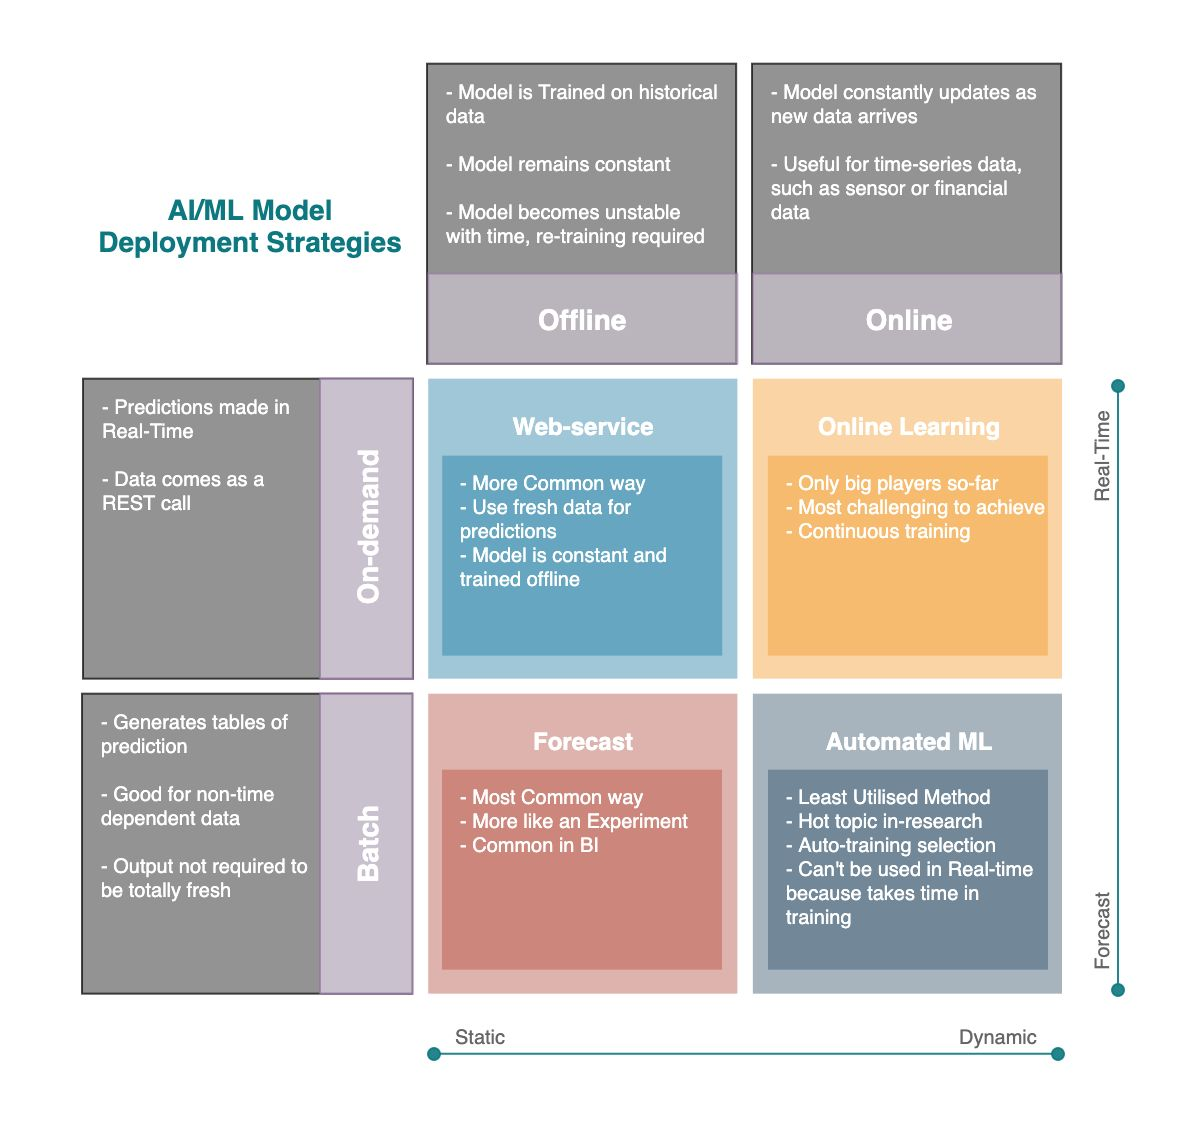
\includegraphics[width=1\textwidth]{images/ml-model-deployment-strategies.jpg}
\caption{ML Model Deployment Strategies}
\label{flask-rq-flow}
\end{figure}



\section{Tables}

\begin{table}[H]
\centering
\begin{tabular}{|l|l|}
row-1, col-1 & row-1, col-2 \\
row-2, col-1 & row-2, col-2 \\
\end{tabular}
\caption{table-A}
\end{table}

\begin{table}[H]
\centering
\begin{tabular}{|l|l|}
row-1, col-1 & row-1, col-2 \\
\hline
row-2, col-1 & row-2, col-2 \\
\cline{1-1}
row-3, col-1 & row-3, col-2 \\
\cline{2-2}
row-4, col-1 & row-4, col-2 \\
\hline \hline
row-5, col-1 & row-5, col-2 \\
\hline
\end{tabular}
\caption{table-B}
\end{table}

\begin{table}[H]
\centering
\begin{tabular}{l|r|l}
Item & Quantity & Price (\$) \\
\hline
Nails & 500 & 0.34 \\
Wooden boards & 100 & 4.00 \\
Bricks & 240 & 11.50 \\
\end{tabular}
\caption{table-C}
\end{table}


\begin{table}[H]
\centering
\begin{tabular}{l|rcll}
& & Year \\
\cline{2-4}
City & 2006 & 2007 & 2008 \\
\hline
London & 45789 & 46551 & 51298 \\
Berlin & 34549 & 32543 & 29870 \\
Paris & 49385 & 51009 & 51970 \\
\end{tabular}
\caption{table-C}
\end{table}

\begin{table}[H]
\centering
\begin{tabular}{|l|l|}
row-1, col-1 & row-1, col-2 \\
row-2, col-1 & row-2, col-2 \\
\end{tabular}
\caption{table-D}
\end{table}

\section{Equations}

$1+2=3$
$$1+2=3$$
\begin{equation}
1+2=3
\end{equation}


\begin{eqnarray*}
a & = & b + c \\
  & = & y - z
\end{eqnarray*}


\begin{eqnarray}
a & = & b + c \\
  & = & y - z
\end{eqnarray}

\section{Tips}

\begin{enumerate}
\item To absolutely force a figure/table to appear “here”, you can \textbackslash usepackage{float} and use the H specifier which it defines
\end{enumerate}

\section{References}

\begin{enumerate}
\item http://www.docs.is.ed.ac.uk/skills/documents/3722/3722-2014.pdf
\item https://texfaq.org/FAQ-figurehere
\item http://detexify.kirelabs.org/
\item http://mirror.iopb.res.in/tex-archive/macros/latex/contrib/natbib/natnotes.pdf
\end{enumerate}

\end{document}
